%!TeX root=../pridetop.tex
\chapter[Chapter \thechapter]{}


\begin{figure}[t!]
\centering
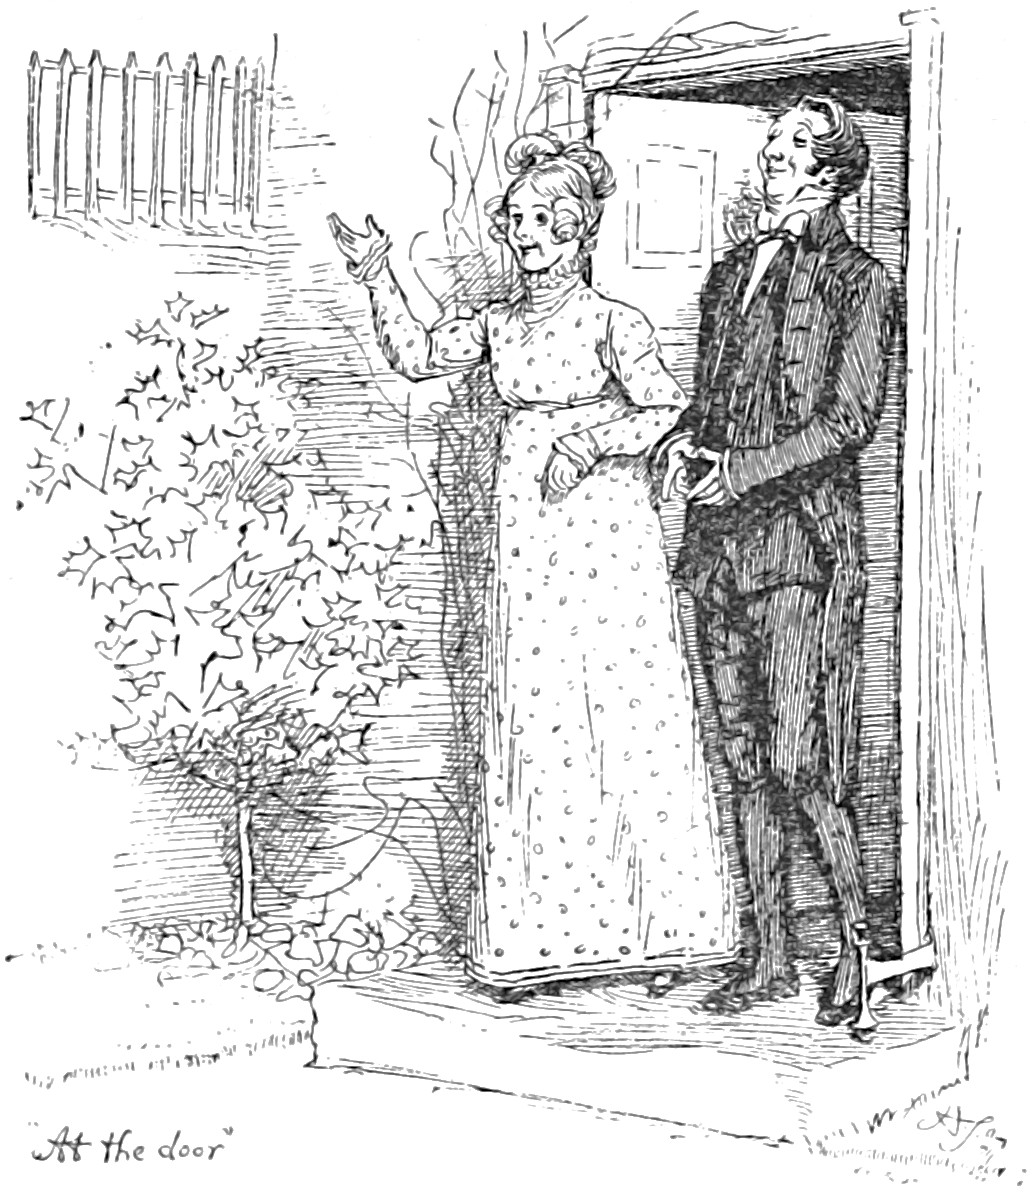
\includegraphics[width=.8\linewidth]{28top}
\captionlistentry{At the door}
\end{figure}


\lettrine[lines=6,image=true]{initials/chap28e}{very}  object in the next day's journey was new and interesting to Elizabeth; and her spirits were in a state of enjoyment; for she had seen her sister looking so well as to banish all fear for her health, and the prospect of her northern tour was a constant source of delight.

\zz
When they left the high road for the lane to Hunsford, every eye was in search of the Parsonage, and every turning expected to bring it in view. The paling of Rosings park was their boundary on one side. Elizabeth smiled at the recollection of all that she had heard of its inhabitants.

At length the Parsonage was discernible. The garden sloping to the road, the house standing in it, the green pales and the laurel hedge, everything declared they were arriving. Mr Collins and Charlotte appeared at the door, and the carriage stopped at the small gate, which led by a short gravel walk to the house, amidst the nods and smiles of the whole party. In a moment they were all out of the chaise, rejoicing at the sight of each other. Mrs Collins welcomed her friend with the liveliest pleasure, and Elizabeth was more and more satisfied with coming, when she found herself so affectionately received. She saw instantly that her cousin's manners were not altered by his marriage: his formal civility was just what it had been; and he detained her some minutes at the gate to hear and satisfy his inquiries after all her family. They were then, with no other delay than his pointing out the neatness of the entrance, taken into the house; and as soon as they were in the parlour, he welcomed them a second time, with ostentatious formality, to his humble abode, and punctually repeated all his wife's offers of refreshment.

Elizabeth was prepared to see him in his glory; and she could not help fancying that in displaying the good proportion of the room, its aspect, and its furniture, he addressed himself particularly to her, as if wishing to make her feel what she had lost in refusing him. But though everything seemed neat and comfortable, she was not able to gratify him by any sigh of repentance; and rather looked with wonder at her friend, that she could have so cheerful an air with such a companion. When Mr Collins said anything of which his wife might reasonably be ashamed, which certainly was not seldom, she involuntarily turned her eye on Charlotte. Once or twice she could discern a faint blush; but in general Charlotte wisely did not hear. After sitting long enough to admire every article of furniture in the room, from the sideboard to the fender, to give an account of their journey, and of all that had happened in London, Mr Collins invited them to take a stroll in the garden, which was large and well laid out, and to the cultivation of which he attended himself. To work in his garden was one of his most respectable pleasures; and Elizabeth admired the command of countenance with which Charlotte talked of the healthfulness of the exercise, and owned she encouraged it as much as possible. Here, leading the way through every walk and cross walk, and scarcely allowing them an interval to utter the praises he asked for, every view was pointed out with a minuteness which left beauty entirely behind. He could number the fields in every direction, and could tell how many trees there were in the most distant clump. But of all the views which his garden, or which the country or the kingdom could boast, none were to be compared with the prospect of Rosings, afforded by an opening in the trees that bordered the park nearly opposite the front of his house. It was a handsome modern building, well situated on rising ground.

From his garden, Mr Collins would have led them round his two meadows; but the ladies, not having shoes to encounter the remains of a white frost, turned back; and while Sir William accompanied him, Charlotte took her sister and friend over the house, extremely well pleased, probably, to have the opportunity of showing it without her husband's help. It was rather small, but well built and convenient; and everything was fitted up and arranged with a neatness and consistency, of which Elizabeth gave Charlotte all the credit. When Mr Collins could be forgotten, there was really a great air of comfort throughout, and by Charlotte's evident enjoyment of it, Elizabeth supposed he must be often forgotten.

She had already learnt that Lady Catherine was still in the country. It was spoken of again while they were at dinner, when Mr Collins joining in, observed,—

<Yes, Miss Elizabeth, you will have the honour of seeing Lady Catherine de Bourgh on the ensuing Sunday at church, and I need not say you will be delighted with her. She is all affability and condescension, and I doubt not but you will be honoured with some portion of her notice when service is over. I have scarcely any hesitation in saying that she will include you and my sister Maria in every invitation with which she honours us during your stay here. Her behaviour to my dear Charlotte is charming. We dine at Rosings twice every week, and are never allowed to walk home. Her Ladyship's carriage is regularly ordered for us. I \textit{should} say, one of her Ladyship's carriages, for she has several.>

<Lady Catherine is a very respectable, sensible woman, indeed,> added Charlotte, <and a most attentive neighbour.>

<Very true, my dear, that is exactly what I say. She is the sort of woman whom one cannot regard with too much deference.>

The evening was spent chiefly in talking over Hertfordshire news, and telling again what had been already written; and when it closed, Elizabeth, in the solitude of her chamber, had to meditate upon Charlotte's degree of contentment, to understand her address in guiding, and composure in bearing with, her husband, and to acknowledge that it was all done very well. She had also to anticipate how her visit would pass, the quiet tenour of their usual employments, the vexatious interruptions of Mr Collins, and the gaieties of their intercourse with Rosings. A lively imagination soon settled it all.

About the middle of the next day, as she was in her room getting ready for a walk, a sudden noise below seemed to speak the whole house in confusion; and, after listening a moment, she heard somebody running upstairs in a violent hurry, and calling loudly after her. She opened the door, and met Maria in the landing-place, who, breathless with agitation, cried out,—

<Oh, my dear Eliza! pray make haste and come into the dining-room, for there is such a sight to be seen! I will not tell you what it is. Make haste, and come down this moment.>

Elizabeth asked questions in vain; Maria would tell her nothing more; and down they ran into the dining-room which fronted the lane, in quest of this wonder; it was two ladies, stopping in a low phaeton at the garden gate.

<And is this all?> cried Elizabeth. <I expected at least that the pigs were got into the garden, and here is nothing but Lady Catherine and her daughter!>

<La! my dear,> said Maria, quite shocked at the mistake, <it is not Lady Catherine. The old lady is Mrs Jenkinson, who lives with them. The other is Miss de Bourgh. Only look at her. She is quite a little creature. Who would have thought she could be so thin and small!>

<She is abominably rude to keep Charlotte out of doors in all this wind. Why does she not come in?>

<Oh, Charlotte says she hardly ever does. It is the greatest of favours when Miss de Bourgh comes in.>

<I like her appearance,> said Elizabeth, struck with other ideas. <She looks sickly and cross. Yes, she will do for him very well. She will make him a very proper wife.>

\begin{figure}[tbh]
\centering
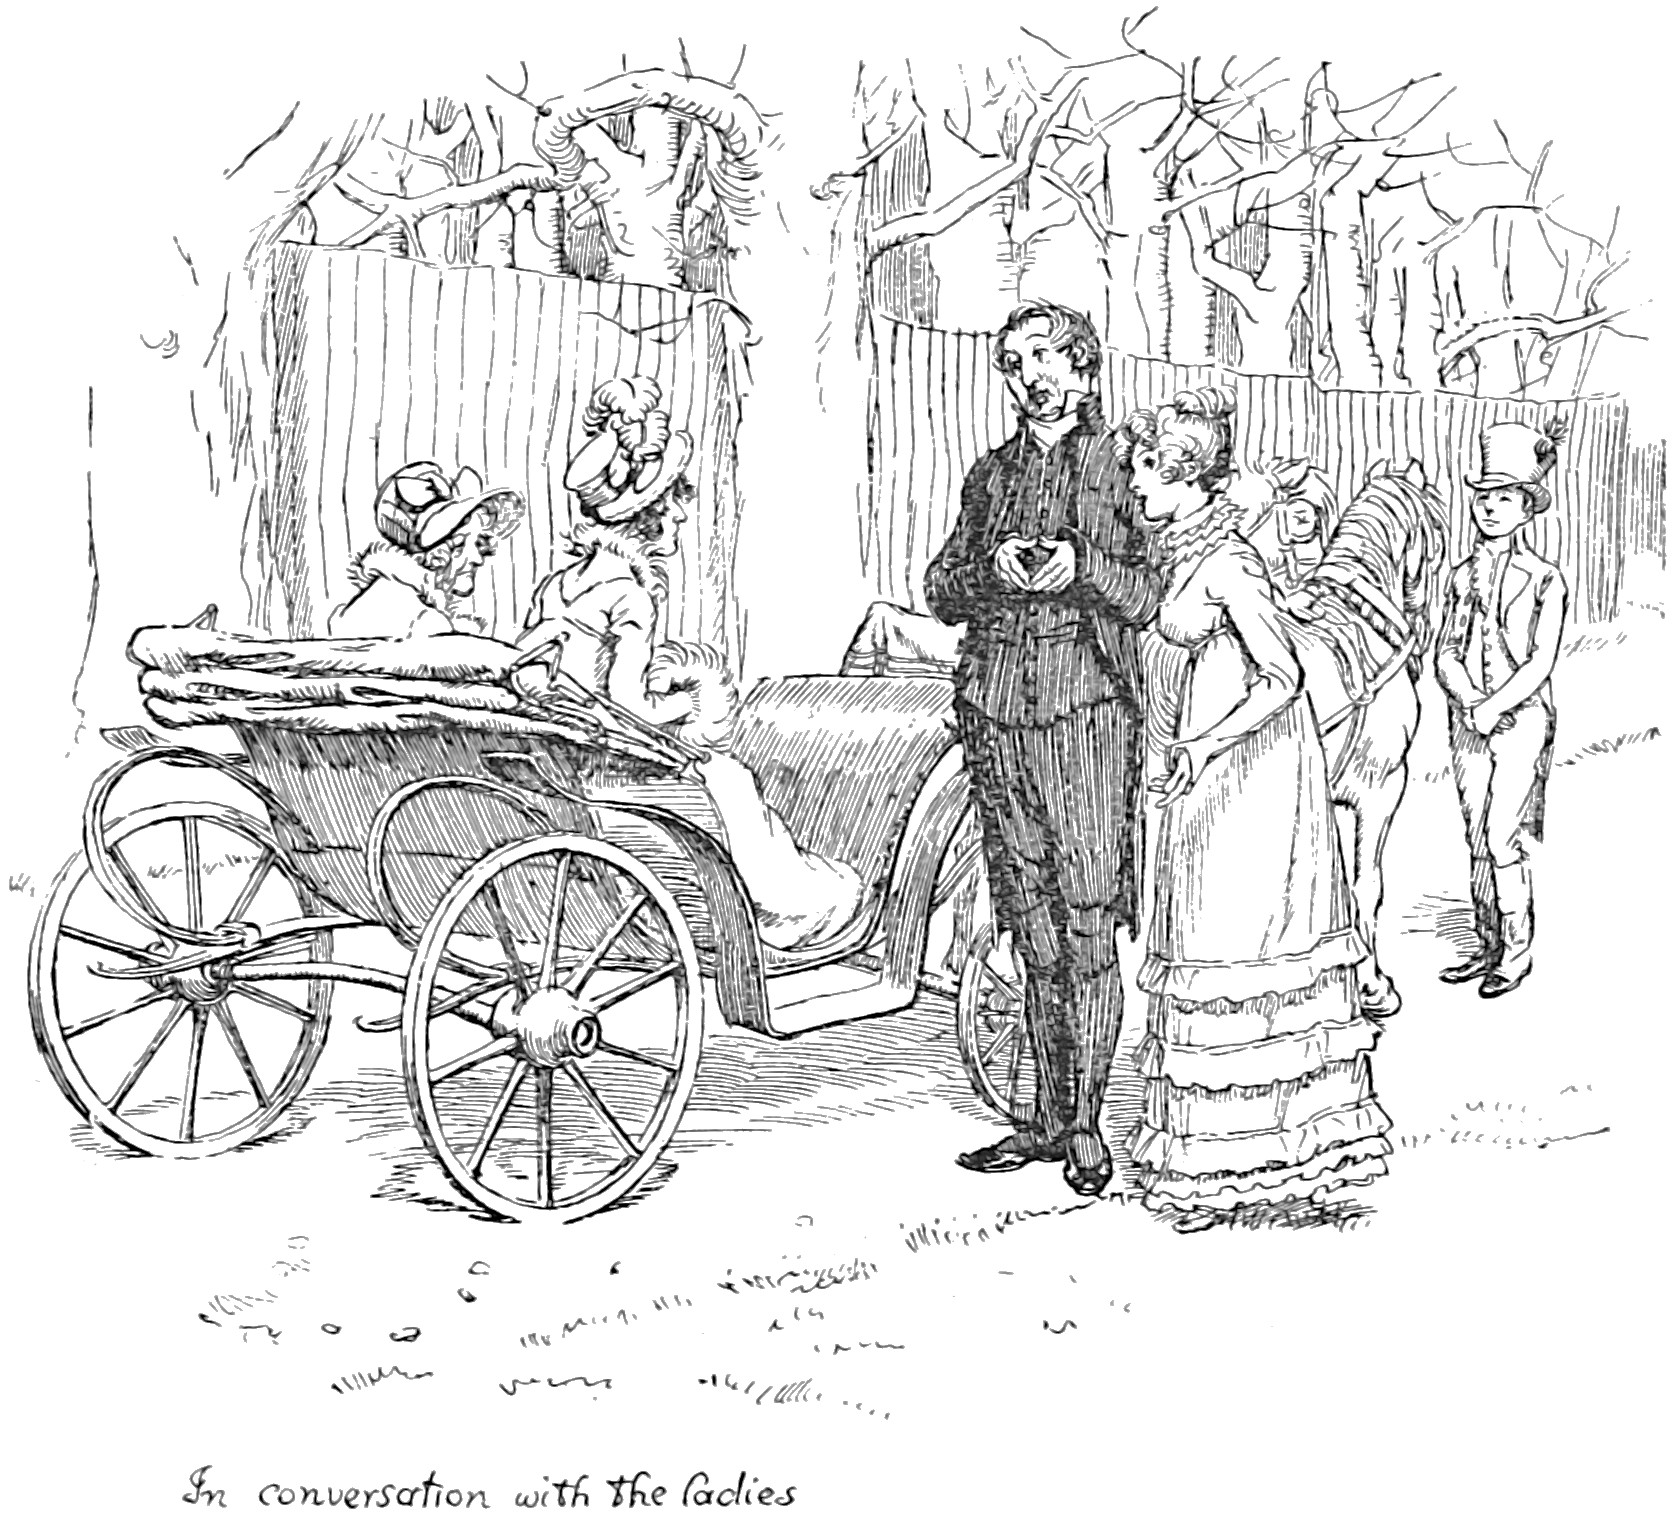
\includegraphics[width=\linewidth]{28conversation}
\captionlistentry{In conversation with the ladies}
\end{figure}

Mr Collins and Charlotte were both standing at the gate in conversation with the ladies; and Sir William, to Elizabeth's high diversion, was stationed in the doorway, in earnest contemplation of the greatness before him, and constantly bowing whenever Miss de Bourgh looked that way.

At length there was nothing more to be said; the ladies drove on, and the others returned into the house. Mr Collins no sooner saw the two girls than he began to congratulate them on their good fortune, which Charlotte explained by letting them know that the whole party was asked to dine at Rosings the next day.